\documentclass[onlymath]{beamer}
% \documentclass[onlymath,handout]{beamer}

% Macros used by all lectures, but not necessarily by excercises

%%% General setup and dependencies:

% \usetheme[ddcfooter,nosectionnum]{tud}
\usetheme[nosectionnum,pagenum,noheader]{tud}
% \usetheme[nosectionnum,pagenum]{tud}

% Increase body font size to a sane level:
\let\origframetitle\frametitle
% \renewcommand{\frametitle}[1]{\origframetitle{#1}\normalsize}
\renewcommand{\frametitle}[1]{\origframetitle{#1}\fontsize{10pt}{13.2}\selectfont}
\setbeamerfont{itemize/enumerate subbody}{size=\small} % tud defaults to scriptsize!
\setbeamerfont{itemize/enumerate subsubbody}{size=\small}
% \setbeamerfont{normal text}{size=\small}
% \setbeamerfont{itemize body}{size=\small}

\renewcommand{\emph}[1]{\textbf{#1}}

\def\arraystretch{1.3}% Make tables even less cramped vertically

\usepackage[ngerman]{babel}
\usepackage[utf8]{inputenc}
\usepackage[T1]{fontenc}

%\usepackage{graphicx}
\usepackage[export]{adjustbox} % loads graphicx
\usepackage{import}
\usepackage{stmaryrd}
\usepackage[normalem]{ulem} % sout command
% \usepackage{times}
\usepackage{txfonts}
\usepackage{array}

% \usepackage[perpage]{footmisc} % reset footnote counter on each page -- fails with beamer (footnotes gone)
\usepackage{perpage}  % reset footnote counter on each page
\MakePerPage{footnote}

\usepackage{tikz}
\usetikzlibrary{arrows,positioning,decorations.pathreplacing}
% Inspired by http://www.texample.net/tikz/examples/hand-drawn-lines/
\usetikzlibrary{decorations.pathmorphing}
\pgfdeclaredecoration{penciline}{initial}{
    \state{initial}[width=+\pgfdecoratedinputsegmentremainingdistance,
    auto corner on length=1mm,]{
        \pgfpathcurveto%
        {% From
            \pgfqpoint{\pgfdecoratedinputsegmentremainingdistance}
                      {\pgfdecorationsegmentamplitude}
        }
        {%  Control 1
        \pgfmathrand
        \pgfpointadd{\pgfqpoint{\pgfdecoratedinputsegmentremainingdistance}{0pt}}
                    {\pgfqpoint{-\pgfdecorationsegmentaspect
                     \pgfdecoratedinputsegmentremainingdistance}%
                               {\pgfmathresult\pgfdecorationsegmentamplitude}
                    }
        }
        {%TO
        \pgfpointadd{\pgfpointdecoratedinputsegmentlast}{\pgfpoint{1pt}{1pt}}
        }
    }
    \state{final}{}
}
\tikzset{handdrawn/.style={decorate,decoration=penciline}}
\tikzset{every shadow/.style={fill=none,shadow xshift=0pt,shadow yshift=0pt}}
% \tikzset{module/.append style={top color=\col,bottom color=\col}}

% Use to make Tikz attributes with Beamer overlays
% http://tex.stackexchange.com/a/6155
\tikzset{onslide/.code args={<#1>#2}{%
  \only<#1| handout:0>{\pgfkeysalso{#2}}
}}
\tikzset{onslideprint/.code args={<#1>#2}{%
  \only<#1>{\pgfkeysalso{#2}}
}}

%%% Title -- always set this first

\newcommand{\defineTitle}[3]{
	\newcommand{\lectureindex}{#1}
	\title{Theoretische Informatik und Logik}
	\subtitle{\href{\lectureurl}{#1. Vorlesung: #2}}
	\author{\href{https://iccl.inf.tu-dresden.de/web/Markus_Kr\%C3\%B6tzsch}{Markus Kr\"{o}tzsch}\\[1ex]Lehrstuhl Wissensbasierte Systeme}
	\date{#3}
	\datecity{TU Dresden}
% 	\institute{CC-By 3.0, sofern keine anderslautenden Bildrechte angegeben sind}
}

%%% Table of contents:

\RequirePackage{ifthen}

\newcommand{\highlight}[2]{%
	\ifthenelse{\equal{#1}{\lectureindex}}{\alert{#2}}{#2}%
}

\def\myspace{-0.7ex}
\newcommand{\printtoc}{
\begin{tabular}{r@{$\quad$}l}
\highlight{1}{1.} & \highlight{1}{Willkommen/Einleitung formale Sprachen}\\[\myspace]
\highlight{2}{2.} & \highlight{2}{Grammatiken und die Chomsky-Hierarchie}\\[\myspace]
\highlight{3}{3.} & \highlight{3}{Endliche Automaten}\\[\myspace]
\highlight{4}{4.} & \highlight{4}{Complexity of FO query answering}\\[\myspace]
\highlight{5}{5.} & \highlight{5}{Conjunctive queries}\\[\myspace]
\highlight{6}{6.} & \highlight{6}{Tree-like conjunctive queries}\\[\myspace]
\highlight{7}{7.} & \highlight{7}{Query optimisation}\\[\myspace]
\highlight{8}{8.} & \highlight{8}{Conjunctive Query Optimisation / First-Order~Expressiveness}\\[\myspace]
\highlight{9}{9.} & \highlight{9}{First-Order~Expressiveness / Introduction to Datalog}\\[\myspace]
\highlight{10}{10.} & \highlight{10}{Expressive Power and Complexity of Datalog}\\[\myspace]
\highlight{11}{11.} & \highlight{11}{Optimisation and Evaluation of Datalog}\\[\myspace]
\highlight{12}{12.} & \highlight{12}{Evaluation of Datalog (2)}\\[\myspace]
\highlight{13}{13.} & \highlight{13}{Graph Databases and Path Queries}\\[\myspace]
\highlight{14}{14.} & \highlight{14}{Outlook: database theory in practice}
\end{tabular}
}

\newcommand{\overviewslide}{%
\begin{frame}\frametitle{Overview}
\printtoc
\medskip

Siehe \href{\lectureurl}{course homepage [$\Rightarrow$ link]} for more information and materials
\end{frame}
}

%%% Colours:
\usepackage{xcolor,colortbl}
\definecolor{redhighlights}{HTML}{FFAA66}
\definecolor{lightblue}{HTML}{55AAFF}
\definecolor{lightred}{HTML}{FF5522}
\definecolor{lightpurple}{HTML}{DD77BB}
\definecolor{lightgreen}{HTML}{55FF55}
\definecolor{darkred}{HTML}{CC4411}
\definecolor{darkblue}{HTML}{176FC0}%{1133AA}
\definecolor{nightblue}{HTML}{2010A0}%{1133AA}
\definecolor{alert}{HTML}{176FC0}
\definecolor{darkgreen}{HTML}{36AB14}
\definecolor{strongyellow}{HTML}{FFE219}
\definecolor{devilscss}{HTML}{666666}

\newcommand{\redalert}[1]{\textcolor{darkred}{#1}}

%%% Slide layout commands:

\newcommand{\sectionSlide}[1]{
\frame{\begin{center}
\LARGE
#1
\end{center}}
}
\newcommand{\sectionSlideNoHandout}[1]{
\frame<handout:0>{\begin{center}
\LARGE
#1
\end{center}}
}

\newcommand{\mydualbox}[3]{%
 \begin{minipage}[t]{#1}
 \begin{beamerboxesrounded}[upper=block title,lower=block body,shadow=true]%
    {\centering\usebeamerfont*{block title}#2}%
    \raggedright%
    \usebeamerfont{block body}
%     \small
    #3%
  \end{beamerboxesrounded}
  \end{minipage}
}
%
\newcommand{\myheaderbox}[2]{%
 \begin{minipage}[t]{#1}
 \begin{beamerboxesrounded}[upper=block title,lower=block title,shadow=true]%
    {\centering\usebeamerfont*{block title}\rule{0pt}{2.6ex} #2}%
  \end{beamerboxesrounded}
  \end{minipage}
}

\newcommand{\mycontentbox}[2]{%
 \begin{minipage}[t]{#1}%
 \begin{beamerboxesrounded}[upper=block body,lower=block body,shadow=true]%
    {\centering\usebeamerfont*{block body}\rule{0pt}{2.6ex}#2}%
  \end{beamerboxesrounded}
  \end{minipage}
}

\newcommand{\mylcontentbox}[2]{%
 \begin{minipage}[t]{#1}%
 \begin{beamerboxesrounded}[upper=block body,lower=block body,shadow=true]%
    {\flushleft\usebeamerfont*{block body}\rule{0pt}{2.6ex}#2}%
  \end{beamerboxesrounded}
  \end{minipage}
}

% label=180:{\rotatebox{90}{{\footnotesize\textcolor{darkgreen}{Beispiel}}}}
% \hspace{-8mm}\ghost{\raisebox{-7mm}{\rotatebox{90}{{\footnotesize\textcolor{darkgreen}{Beispiel}}}}}\hspace{8mm}
\newcommand{\examplebox}[1]{%
	\begin{tikzpicture}[decoration=penciline, decorate]
		\pgfmathsetseed{1235}
		\node (n1) [decorate,draw=darkgreen, fill=darkgreen!10,thick,align=left,text width=\linewidth, inner ysep=2mm, inner xsep=2mm] at (0,0) {#1};
% 		\node (n2) [align=left,text width=\linewidth,inner sep=0mm] at (n1.92) {{\footnotesize\raisebox{3mm}{\textcolor{darkgreen}{Beispiel}}}};
% 		\node (n2) [decorate,draw=darkgreen, fill=darkgreen!10,thick, align=left,text width=\linewidth,inner sep=2mm] at (n1.90) {{\footnotesize\raisebox{0mm}{\textcolor{darkgreen}{Beispiel}}}};
	\end{tikzpicture}%
}%

\newcommand{\codebox}[1]{%
	\begin{tikzpicture}[decoration=penciline, decorate]
		\pgfmathsetseed{1236}
		\node (n1) [decorate,draw=strongyellow, fill=strongyellow!10,thick,align=left,text width=\linewidth, inner ysep=2mm, inner xsep=2mm] at (0,0) {#1};
	\end{tikzpicture}%
}%

\newcommand{\defbox}[1]{%
	\begin{tikzpicture}[decoration=penciline, decorate]
		\pgfmathsetseed{1237}
		\node (n1) [decorate,draw=darkred, fill=darkred!10,thick,align=left,text width=\linewidth, inner ysep=2mm, inner xsep=2mm] at (0,0) {#1};
	\end{tikzpicture}%
}%

\newcommand{\theobox}[1]{%
	\begin{tikzpicture}[decoration=penciline, decorate]
		\pgfmathsetseed{1240}
		\node (n1) [decorate,draw=darkblue, fill=darkblue!10,thick,align=left,text width=\linewidth, inner ysep=2mm, inner xsep=2mm] at (0,0) {#1};
	\end{tikzpicture}%
}%

\newcommand{\anybox}[2]{%
	\begin{tikzpicture}[decoration=penciline, decorate]
		\pgfmathsetseed{1240}
		\node (n1) [decorate,draw=#1, fill=#1!10,thick,align=left,text width=\linewidth, inner ysep=2mm, inner xsep=2mm] at (0,0) {#2};
	\end{tikzpicture}%
}%


\newsavebox{\mybox}%
\newcommand{\doodlebox}[2]{%
\sbox{\mybox}{#2}%
	\begin{tikzpicture}[decoration=penciline, decorate]
		\pgfmathsetseed{1238}
		\node (n1) [decorate,draw=#1, fill=#1!10,thick,align=left,inner sep=1mm] at (0,0) {\usebox{\mybox}};
	\end{tikzpicture}%
}%


\defineTitle{20}{Resolution/Endliche Modelle}{30. Juni 2017}

\begin{document}

\maketitle

\frame{\label{frame_herbrand}\begin{center}
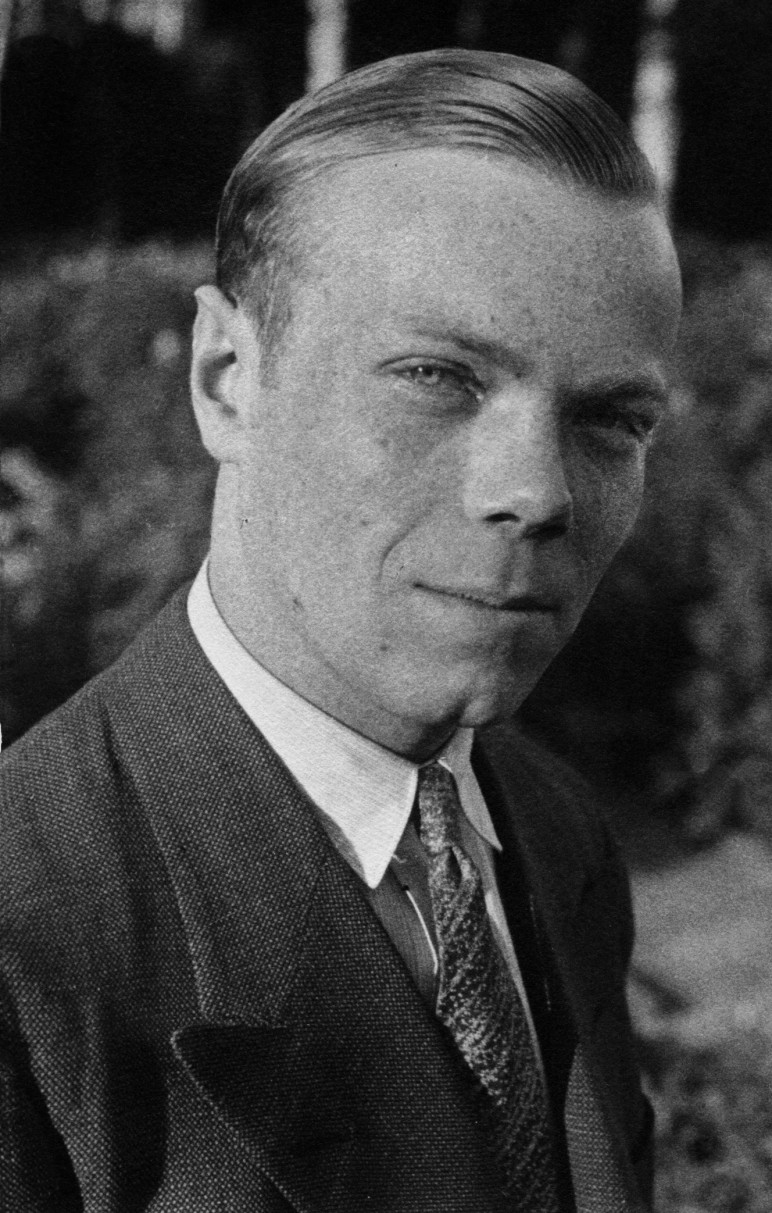
\includegraphics[height=5cm]{images/Herbrand.jpg}

\LARGE
Jacques Herbrand\medskip

\normalsize
12.2.1908 -- 27.7.1931
\end{center}}

\begin{frame}\frametitle{Resolution}

Resolutionsregel:
\[  \frac{
\{A_1,\ldots,A_n,L_1,\ldots,L_k\}\quad
\{\neg A'_1,\ldots,\neg A'_m,L'_1,\ldots,L'_\ell\}
}{\{L_1\sigma,\ldots,L_k\sigma,L'_1\sigma,\ldots,L'_\ell\sigma\}
}\]
falls $\sigma$ allgemeinster Unifikator von $\{A_1,\ldots,A_n, A'_1,\ldots, A'_m\}$ ist\bigskip

\emph{Algorithmus (Skizze):}
\begin{enumerate}[(1)]
\item Bilde Klauselform
\item Bilde systematisch Resolventen durch Resolution von Varianten bereits abgeleiteter Klauseln
\item Wiederhole (2), bis entweder $\bot$ erzeugt wird ("`unerfüllbar"') oder keine neuen Klauseln mehr entstehen\footnote{Dieser Fall ist eher ungewöhnlich: Meist entstehen bei erfüllbaren Theorien immer mehr neue Klauseln ohne dass das Verfahren terminiert.}
\end{enumerate}

\end{frame}

\begin{frame}\frametitle{Vollständigkeit und Korrektheit}

\theobox{Resolutionssatz: Sei $F$ eine prädikatenlogische Formel und $\mathcal{K}_i$ ($i\geq 0$) die vom Resolutionsalgorithmus ermittelten Klauselmengen. Dann sind die folgenden Aussagen äquivalent:
\begin{itemize}
\item $F$ ist unerfüllbar
\item Es gibt ein $\ell\geq 0$ mit $\bot\in\mathcal{K}_\ell$
\end{itemize}}

\begin{itemize}
\item Korrektheit hatten wir bereits gezeigt
\item Vollständigkeit steht noch aus
\end{itemize}

\end{frame}

\begin{frame}\frametitle{Korrektheit (Korrektur)}

\emph{Beweis (Korrektheit Resoutionsschritt):} Gegeben:
\begin{itemize}
\item Klauseln $K_1=\{A_1,\ldots,A_n,L_1,\ldots,L_k\}$ und $K_2=\{\neg A'_1,\ldots,\neg A'_m,L'_1,\ldots,L'_\ell\}$
\item (allgemeinster) Unifikator $\sigma$ der Menge $\{A_1,\ldots,A_n,A'_1,\ldots,A'_m\}$
\item zugehörige Resolvente $K=\{L_1\sigma,\ldots,L_k\sigma,L'_1\sigma,\ldots, L'_\ell\sigma\}$\pause
\end{itemize}

Sei $\Inter$ eine beliebige Interpretation.
\begin{itemize}
\item Falls $\Inter\models\forall K_1\wedge\forall K_2$, dann gilt auch $\Inter\models\forall (K_1\sigma)\wedge\forall (K_2\sigma)$ (die Substitution konkretisiert eine Allaussage)
\item Also gilt für alle Zuweisungen $\Zuweisung$: $\Inter,\Zuweisung\models(K_1\sigma)\wedge (K_2\sigma)$
\item Fall 1: $\Inter,\Zuweisung\models A_1\sigma$ ($=A_2\sigma=\ldots=A'_m\sigma)$. Dann gilt $\Inter,\Zuweisung\models L'_1\sigma\vee\ldots\vee L'_\ell\sigma$, und damit $\Inter,\Zuweisung\models K$
\item Fall 2: $\Inter,\Zuweisung\not\models A_1\sigma$ ($=A_2\sigma=\ldots=A'_m\sigma)$. Dann gilt $\Inter,\Zuweisung\models L_1\sigma\vee\ldots\vee L_k\sigma$, und damit $\Inter,\Zuweisung\models K$
\item Also gilt $\Inter\models\forall K$.
\end{itemize}
Da $\Inter$ beliebig ist gilt also $\forall K_1\wedge\forall K_2\models \forall K$
-- d.h., jede Resolvente ist logische Konsequenz der resolvierten Klauseln

\end{frame}

\sectionSlide{Prädikatenlogisches Schließen mit Aussagenlogik}

\begin{frame}\frametitle{Herbrand-Expansionen}

\defbox{Die \redalert{Herbrand-Expansion} $HE(F)$ einer Formel $F=\forall x_1,\ldots, x_n.G$ in Skolemform ist die Menge:
\[ HE(F)\defeq\big\{ G\{x_1\mapsto t_1,\ldots,x_n\mapsto t_n\}\mid t_1,\ldots,t_n\in\Delta_F\big\}\]
}

$HE(F)$ ist also die (möglicherweise unendliche) Menge von \ghost{variablen-}\\ freien Sätzen, die in Herbrandmodellen von $F$ gelten müssten.
\pause\bigskip

\redalert{Quantorenfreie Sätze = aussagenlogische Formeln:}
\begin{itemize}
\item $HE(F)$ enthält Formeln ohne Variablen, d.h. Boolsche Kombinationen geschlossener Atome
\item Geschlossene Atome können unabhängig voneinander wahr oder falsch sein, egal wie ihre genaue Struktur aussieht
\item Wir können sie also als "`ungewöhnlich benannte"' aussagenlogische Atome auffassen und die gesamte Formel aussagenlogisch interpretieren
\end{itemize}
\alert{$\leadsto$ $HE(F)$ als aussagenlogische Theorie}


\end{frame}

\begin{frame}\frametitle{Gödel, Herbrand, Skolem}

\theobox{Satz von Gödel, Herbrand \& Skolem: Eine Formel $F$ in Skolemform ist genau dann erfüllbar, wenn $HE(F)$ aussagenlogisch erfüllbar ist.}\pause

\emph{Beweis:} Wir zeigen, dass $F=\forall x_1,\ldots,x_n.G$ genau dann ein Herbrandmodell hat, wenn $HE(F)$ aussagenlogisch erfüllbar ist:\pause

\begin{itemize}
\item $\Inter$ ist ein Herbrandmodell von $F$\pause
\item gdw. $\Inter,\{x_1\mapsto t_1,\ldots,x_n\mapsto t_n\}\models G$ für alle $t_1,\ldots,t_n\in\Delta_F$\pause
\item gdw. $\Inter\models G\{x_1\mapsto t_1,\ldots,x_n\mapsto t_n\}$ für alle $t_1,\ldots,t_n\in\Delta_F$ (Lemma)\pause
\item gdw. für alle $H\in HE(F)$ gilt $\Inter\models H$\pause
\item gdw. $\Inter$ als aussagenlogisches Modell für $HE(F)$ angesehen werden kann.\qed
\end{itemize}

\end{frame}

\begin{frame}\frametitle{Satz von Herbrand}

Als Korollar der gezeigten Ergebnisse erhalten wir ein wichtiges Resultat:

\theobox{Satz: Eine Formel $F$ in Skolemform ist genau dann unerfüllbar, wenn
eine endliche Teilmenge von $E(F)$ aussagenlogisch unerfüllbar ist.}

\pause\emph{Beweis:} Das Kontrapositiv des Satzes von Gödel, Herbrand \& Skolem besagt:\medskip

Eine Formel $F$ in Skolemform ist genau dann unerfüllbar, wenn $HE(F)$ aussagenlogisch unerfüllbar ist.\bigskip

Der Satz folgt nun, weil jede unerfüllbare aussagenlogische Formelmenge eine endliche
Teilmenge hat, die unerfüllbar ist (Kompaktheit der Aussagenlogik, siehe Formale Systeme, WS 2016/2017, Vorlesung 24)\qed

\end{frame}

\begin{frame}\frametitle{Prädikatenlogik semi-entscheiden}

Das Ergebnis Herbrands ermöglicht bereits einen naiven Algorithmus zur Semi-Entscheidung von Unerfüllbarkeit in der Prädikatenlogik:\bigskip

\emph{Gegeben:} Eine Formel $F$
\begin{itemize}
\item Wandle $F$ in Skolemform $F'$ um
\item Definiere eine Reihenfolge der Formeln in $HE(F')$: $F_1,F_2,F_3,\ldots$
\item Für alle $i\geq 1$:
	\begin{itemize}
	\item Prüfe ob die endliche Menge $\{F_1,\ldots, F_i\}$ aussagenlogisch unerfüllbar ist
	\item Falls ja, dann gib "`unerfüllbar"' aus; andernfalls fahre fort
	\end{itemize}
\end{itemize}

Offenbar ist das \redalert{kein praktischer Algorithmus}, aber er zeigt Semi-Entscheidbarkeit

\end{frame}

\sectionSlide{Vollständigkeit der Resolution}

\begin{frame}\frametitle{Ansatz}

\alert{Herbrands Satz liefert uns auch eine Strategie zum Beweis der Vollständigkeit des Resolutionsalgorithmus}\bigskip

\emph{Wir wissen bereits:}
\begin{itemize}
\item Unerfüllbarkeit einer Klauselmenge zeigt sich in der Unerfüllbarkeit ihrer Herbrand-Expansion
\item Die Unerfüllbarkeit der Herbrand-Expansion kann man mit aussagenlogischer Resolution beweisen
\item Prädikatenlogische Resolution verallgemeinert aussagenlogische Resolution indem wir direkt mit Klauseln arbeiten, die noch Variablen enthalten
\end{itemize}\pause

\emph{Frage:} Kann man alle Schlüsse, die man auf expandierten Formeln aussagenlogisch erzeugen kann, auch direkt prädikatenlogisch (mit Variablen) erhalten?

\end{frame}

\begin{frame}\frametitle{Lifting-Lemma}

Wir zeigen: Ja, jeder aussagenlogische Schluss (auf der Expansion) kann auf einen prädikatenlogischen Schluss (auf den Klauseln mit Variablen) "`angehoben"' werden\medskip

\theobox{Satz (Lifting-Lemma): Seien $K_1$ und $K_2$ prädikatenlogische Klauseln mit
Grundinstanzen $K'_1=K_1\sigma$ und $K'_2=K_2\sigma$.${^1}$\bigskip

Wenn $R'$ eine (aussagenlogische) Resolvente von $K'_1$ und $K'_2$ ist, dann gibt es
eine prädikatenlogische Resolvente $R$, welche $R'$ als Grundinstanz hat.
}

\color{devilscss}
{\footnotesize ${^1}$ Die Verwendung der selben Substitution für $K'_1$ und $K'_2$ ist keine Einschränkung, da wir durch Variantenbildung sicherstellen können, dass $K_1$ und $K_2$ keine Variablen gemein haben.

}

\end{frame}

\begin{frame}\frametitle{Lifting-Lemma: Beweis}

\theobox{Satz (Lifting-Lemma): Seien $K_1$ und $K_2$ prädikatenlogische Klauseln mit
Grundinstanzen $K'_1=K_1\sigma$ und $K'_2=K_2\sigma$.\smallskip

Wenn $R'$ eine (aussagenlogische) Resolvente von $K'_1$ und $K'_2$ ist, dann gibt es
eine prädikatenlogische Resolvente $R$, welche $R'$ als Grundinstanz hat.
}

\emph{Beweis:} Sei $A'\in K'_1$ das (geschlossene) Atom, über das resolviert wurde, d.h. $\neg A'\in K'_2$.\smallskip\pause

Sei $\mathcal{A}_1\defeq\{A\mid A\in K_1,\;A\sigma=A'\}$ und $\mathcal{A}_2\defeq\{A\mid \neg A\in K_2, A\sigma=A'\}$.\smallskip\pause

Dann ist $\sigma$ ein Unifikator für $\mathcal{A}_1\cup\mathcal{A}_2$.\\ Also hat $\mathcal{A}_1\cup\mathcal{A}_2$ einen allgemeinsten Unifikator $\theta$.\smallskip\pause

Sei $R$ die Resolvente von $K_1$ und $K_2$ bzgl. $\theta$.\smallskip\pause

Dann enthalten $R'$ und $R$ Instanzen der gleichen Literale, d.h. sie sind von der Form
$R'=\{L_1\sigma,\ldots,L_n\sigma\}$ und $R=\{L_1\theta,\ldots,L_n\theta\}$\smallskip\pause

Da $\theta$ allgemeinster Unifikator ist gibt es $\lambda$ mit $\sigma=\theta\circ\lambda$
und es gilt: $R\lambda=\{L_1\theta\lambda,\ldots,L_n\theta\lambda\}=\{L_1\sigma,\ldots,L_n\sigma\}=R'$\qed


\end{frame}


\begin{frame}[t]\frametitle{Vollständigkeit der Resolution (1)}

\theobox{Resolutionssatz: Sei $F$ eine prädikatenlogische Formel und $\mathcal{K}_i$ ($i\geq 0$) die vom Resolutionsalgorithmus ermittelten Klauselmengen. Dann sind die folgenden Aussagen äquivalent:
\begin{itemize}
\item $F$ ist unerfüllbar
\item Es gibt ein $\ell\geq 0$ mit $\bot\in\mathcal{K}_\ell$
\end{itemize}}\pause

\emph{Beweis (Vollständigkeit):} Sei $F$ unerfüllbar
\begin{itemize}
\item Dann ist $HE(F)$ unerfüllbar
\item Dann gibt es eine (endliche) aussagenlogische Resolutionsableitung von $\bot$ aus $HE(F)$
\item Die Ableitung erzeugt eine endliche Folge von Klauseln: $K_1',K_2',\ldots,K_{m-1}',K_m'=\bot$
\item \alert{Behauptung:} Jede Klausel $K_i'$ ist Grundinstanz einer Klausel $K_i$ die in $\mathcal{K}_\ell$ vorkommt für ein $\ell\geq 0$.
\item Für $i=m$ folgt daraus der Satz, denn $K_m'=\bot$ kann nur Grundinstanz von $\bot$ sein, d.h. $\bot\in\mathcal{K}_\ell$ für ein $\ell\geq 0$.
\end{itemize}

\end{frame}

\begin{frame}[t]\frametitle{Vollständigkeit der Resolution (2)}

% \theobox{Resolutionssatz: Sei $F$ eine prädikatenlogische Formel und $\mathcal{K}_i$ ($i\geq 0$) die vom Resolutionsalgorithmus ermittelten Klauselmengen. Dann sind die folgenden Aussagen äquivalent:
% \begin{itemize}
% \item $F$ ist unerfüllbar
% \item Es gibt ein $\ell\geq 0$ mit $\bot\in\mathcal{K}_\ell$
% \end{itemize}}

\emph{Beweis (Vollständigkeit):} \alert{Behauptung:} Jede Klausel $K_i'$ ist Grundinstanz einer Klausel $K_i$ die in $\mathcal{K}_\ell$ vorkommt für ein $\ell\geq 0$.
\medskip\pause

Aussage klar für $K'_i\in HE(F)$: in diesem Fall ist $K'_i$ ist Grundinstanz einer Klausel $K_i$ in der Klauselform von $F$ und in $\mathcal{K}_0$\medskip\pause

Restlicher Beweis durch Induktion über $i$:
\begin{itemize}
\item Indukstionsannahme: Die Aussage gilt für alle $j<i$\pause
\item $K'_i$ ist Resolvente zweier Klauseln $K'_a$ und $K'_b$ mit $a,b<i$\pause
\item Laut Hypothese sind $K'_a$ und $K'_b$ also Instanzen von Klauseln $K_a$ und $K_b$ in einer Menge $\mathcal{K}_\ell$\pause
\item Laut Lifting-Lemma ist demnach $K'_i$ ebenfalls die Instanz einer Klausel $K_i$, die durch Resolution aus $K_a$ und $K_b$ entsteht\pause
\item Diese Resolvente $K_i$ ist also ebenfalls in einer Menge der Form $\mathcal{K}_{\ell'}$\qed
\end{itemize}

\end{frame}

\begin{frame}\frametitle{Kompaktheit}

Die Existenz von vollständigen und korrekten logischen Schließverfahren wie Resolution
ist eng verwandt mit einer grundsätzlichen Eigenschaft der Prädikatenlogik:\bigskip

\theobox{Satz (Endlichkeitssatz, Kompaktheitssatz): Falls eine unendliche Menge prädikatenlogischer Sätze $\mathcal{T}$ eine logische Konsequenz $F$ hat, so ist $F$ auch Konsequenz einer endlichen Teilmenge von $\mathcal{T}$.}\pause

\small
\emph{Beweis:} Die gegebene logische Konsequenz ist gleichbedeutend damit, dass
$\mathcal{T}\cup\{\neg F\}$ unerfüllbar ist.\medskip

Laut Resolutionssatz (Vollständigkeit) kann die Unerfüllbarkeit von $\mathcal{T}\cup\{\neg F\}$ nach endlich vielen Schritten durch Ableitung der leeren Klausel nachgewiesen werden.\medskip

Dabei können nur endlich viele Klauseln aus der Klauselform von $\mathcal{T}\cup\{\neg F\}$ verwendet worden sein. Laut Resolutionssatz (Korrektheit) folgt die Konsequenz also bereits aus einer endlichen Teilmenge von $\mathcal{T}$.\qed

\end{frame}

\begin{frame}\frametitle{Die Grenzen der Prädikatenlogik}

Kompaktheit zeigt uns auch erste Grenzen der Prädikatenlogik auf.
\smallskip

\defbox{Eine logische Formel $F$ mit zwei freien Variablen $x$ und $y$ drückt den \redalert{transitiven Abschluss} einer binären Relation $r$ aus, wenn in jeder Interpretation $\Inter$ und für alle $\delta_1,\delta_2\in\Delta^\Inter$ gilt:\\[1ex]
\narrowcentering{$ \Inter,\{x\mapsto \delta_1,y\mapsto\delta_2\}\models F \quad\text{gdw.}\quad \tuple{\delta_1,\delta_2}\in (r^\Inter)^* $}
}\pause

\theobox{Satz: Es gibt keine prädikatenlogische Formel, die den transitiven Abschluss einer binären Relation ausdrückt.}\pause

\emph{Beweis:} Angenommen es gäbe so eine Formel $F$.\medskip

Dann ist die folgende unendliche Theorie unerfüllbar:
\[\begin{array}{rll}
\big\{ & F\{x\mapsto a,y\mapsto b\},\neg r(a,b), \neg \exists x_1.(r(a,x_1)\wedge r(x_1,b)),\\
& \neg\exists x_1,x_2.(r(a,x_1)\wedge
r(x_1,x_2)\wedge r(x_2,b)),\ldots & \big\}
\end{array}\]
Aber jede endliche Teilmenge der Theorie ist erfüllbar.
Die Existenz der Theorie würde also dem Endlichkeitssatz widersprechen.\qed

\end{frame}


\sectionSlide{Endliche Modelle}

\begin{frame}\frametitle{Endlichkeit von Modellen}

\alert{Löwenheim-Skolem}: Jede erfüllbare Formel hat ein abzählbar großes Modell
\bigskip

\redalert{Kann man dies noch verstärken? Hat jede erfüllbare Formel vielleicht sogar ein endliches Modell?}\pause\bigskip

\alert{Nein! Prädikatenlogik kann unendliche Modelle erzwingen:}\medskip

\examplebox{Beispiel:\vspace{-2ex}
\begin{align*}
\forall x.&(\textsf{Mensch}(x) \to\exists y.(\textsf{hatMutter}(x,y)\wedge\textsf{Mensch}(y))) \\
\forall x,y.&(\textsf{hatMutter}(x,y) \to\textsf{hatVorfahre}(x,y))\\
\forall x,y,z.&((\textsf{hatVorfahre}(x,y)\wedge\textsf{hatVorfahre}(y,z))\to\textsf{hatVorfahre}(x,z))\\
\forall x.&\neg \textsf{hatVorfahre}(x,x)
\end{align*}
Diese Theorie ist erfüllbar, aber hat nur unendliche Modelle.\\ (Kontrollfrage: Warum?)
}

\end{frame}

\begin{frame}\frametitle{Logik über endlichen Modellen}

Sind unendliche Modelle in der Praxis überhaupt wünschenswert?\\
Geht es auch endlich?
\bigskip\pause

\defbox{\redalert{Prädikatenlogik mit endlichen Modellen} verwendet die gleiche Syntax und Semantik wie Prädikatenlogik allgemein, aber mit der zusätzlichen Bedingung, dass die Domäne von Interpretationen endlich sein muss.}\pause

\emph{Monotonie (Rückblick):} weniger Modelle $=$ mehr Konsequenzen

\examplebox{Beispiel:\vspace{-2ex}
\begin{align*}
\forall x.&(\textsf{Mensch}(x) \to\exists y.(\textsf{hatVorfahre}(x,y)\wedge\textsf{Mensch}(y))) \\
% \forall x,y.&(\textsf{hatMutter}(x,y) \to\textsf{hatVorfahre}(x,y))\\
\forall x,y,z.&((\textsf{hatVorfahre}(x,y)\wedge\textsf{hatVorfahre}(y,z))\to\textsf{hatVorfahre}(x,z))
\end{align*}\vspace{-4ex}

Diese Theorie ist in der Prädikatenlogik mit endlichen Modellen erfüllbar, aber jedes endliche Modell muss einen $\textsf{hatVorfahre}$-Zyklus enthalten. Daher folgt
$\exists x.\textsf{hatVorfahre}(x,x)$, obwohl dies in der allgemeinen Prädikatenlogik keine Konsequenz wäre.
}

\end{frame}

\begin{frame}\frametitle{Erfüllbarkeit wird semi-entscheidbar}

Die Bezeichnung der Elemente einer Interpretationsdomäne ist irrelevant -- für die Wahrheit von Sätzen kommt es nur darauf an, wie Konstanten und Prädikatsymbole interpretiert werden.\bigskip\pause

\anybox{strongyellow}{\redalert{Erfüllbarkeitstest}\\[1ex]
\emph{Gegeben:} Ein Satz $F$
\begin{itemize}
\item Betrachte systematisch alle endlichen Interpretationen der Symbole in $F$ (z.B. geordnet nach aufsteigender Größe der Domäne)
\item Prüfe für jedes Modell $\Inter$, ob $\Inter\models F$ gilt:
\begin{itemize}
\item Falls ja, dann gib aus "`erfüllbar"'
\item Falls nein, dann fahre mit nächster Interpretation fort
\end{itemize}
\end{itemize}
}

Es ist leicht zu sehen, dass dieser Algorithmus die Erfüllbarkeit in endlichen Modellen semi-entscheidet.

\end{frame}

\begin{frame}\frametitle{Endlich = einfach?}\pause

Trotzdem bleibt logisches Schließen schwer:

\theobox{Satz von Trakhtenbrot: Logisches Schließen (Erfüllbarkeit, Allgemeingültigkeit, logische Konsequenz) in der Prädikatenlogik mit endlichen Modellen ist unentscheidbar.}

(ohne Beweis)\pause\bigskip

\theobox{Korollar: Es gibt kein vollständiges und korrektes Beweissystem für Prädikatenlogik mit endlichen Modellen.}

\emph{Beweis:} Angenommen es gäbe ein solches System.\pause{} Dann wäre logische Konsequenz und speziell auch Unerfüllbarkeit semi-entscheidbar.\bigskip\pause

Wir wissen, dass Erfüllbarkeit ebenfalls semi-entscheidbar ist.\bigskip\pause

Zusammen ergäbe sich also ein Entscheidungsverfahren für logisches Schließen -- Widerspruch zu Trakhtenbrot.
\qed

\end{frame}

\sectionSlide{Endliche Modelle in der Praxis}

\begin{frame}\frametitle{Wozu endliche Modelle}

In gewisser Weise ist Schließen mit endlichen Modellen also schwerer als mit unendlichen, weil man statt logischer Konsequenz nunmehr nur Nicht-Konsequenz semi-entscheiden kann
\bigskip

Trotzdem sind endliche Interpretationen in der Informatik praktisch relevant:\medskip

\anybox{purple}{Eine endliche Interpretation $\Inter$ ist (im Wesentlichen) das gleiche wie eine \redalert{relationale Datenbankinstanz}.
}
\emph{Intuition:}
\begin{itemize}
\item Prädikatsymbole $p$ bezeichnen Tabellen
\item Relationen $p^\Inter$ entsprechen den in der Datenbank gespeicherten Tabelleninhalten
\end{itemize}

\end{frame}

\begin{frame}\frametitle{Benannte Parameter}

Relationale Datenbanken verwenden \redalert{Namen für die Parameter} (Spalten) in Relationen,
anstatt sie mittels Reihenfolge zu addressieren:\bigskip

\scriptsize

\begin{tabular}[t]{|l|l|}
\multicolumn{2}{@{}l}{linien:}\\
\hline
\textbf{Linie} & \textbf{Typ} \\
\hline
85 & Bus \\\hline
3 & Tram \\\hline
F1 & Fähre \\\hline
\ldots & \ldots\\\hline
\end{tabular}
\hspace{15mm}
\begin{tabular}[t]{|l|l|l|}
\multicolumn{2}{@{}l}{haltestellen:}\\
\hline
\textbf{SID} & \textbf{Name} & \textbf{Rollstuhl}\\
\hline
17 & Hauptbahnhof & true\\\hline
42 & Helmholtzstr. & true\\\hline
57 & Stadtgutstr. & true\\\hline
123 & Gustav-Freytag-Str. & false\\\hline
\ldots & \ldots & \ldots\\\hline
\end{tabular}

\begin{tabular}[t]{|l|l|l|}
\multicolumn{2}{@{}l}{verbindung:}\\
\hline
\textbf{Von} & \textbf{Zu} & \textbf{Linie}\\
\hline
57  & 42 & 85 \\\hline
17  & 789 & 3 \\\hline
\ldots & \ldots & \ldots\\\hline
\end{tabular}
\hspace{0.5cm}
% 
% \medskip
\ghost{
\begin{minipage}[t]{7cm}
\vspace{0.0cm}
Die einfache Arität der Prädikatenlogik wird durch ein\\ \redalert{Schema} mit Namen (und oft auch Datentypen) ersetzt:
\begin{itemize}
\item linien[Linie:string, Typ:string]
\item haltestellen[SID:int, Halt:string, Rollstuhl:bool]
\item verbindung[Von:int, Zu:int, Linie:string]
\end{itemize}
\end{minipage}}

\end{frame}

\begin{frame}\frametitle{Formeln = Anfragen}

Benannt oder nicht -- sofern die Parameter eine definierte Reihenfolge haben,
kann man sie mit normalen prädikatenlogischen Atomen addressieren.\medskip

\examplebox{Beispiel: Die Formel \[Q=\exists z_{\text{Linie}}.(\textsf{verbindung}(x_\text{Von},x_\text{Zu}, z_{\text{Linie}})\wedge \textsf{linien}(z_{\text{Linie}},x_{\text{Typ}}))\]
hat drei freie Variablen. Für eine gegebene Datenbankinstanz (eindliche Interpretation) $\Inter$ bedeutet $\Inter,\{x_\text{Von}\mapsto\delta_1,x_\text{Zu}\mapsto\delta_2,x_\text{Typ}\mapsto\delta_3\}\models Q$, dass es in der Datenbank eine Verbindung von $\delta_1$ nach $\delta_2$ vom Typ $\delta_3$ gibt.
}\pause

Das Beispiel illustriert:
\begin{center}
\large
\redalert{Formeln (ev. mit freien Variablen) = Datenbankanfragen}\\[1ex]
\redalert{Erfüllende Zuweisungen = Anfrage-Ergebnisse}\\
\end{center}
\end{frame}


\begin{frame}\frametitle{Prädikatenlogik $\approx$ SQL}

\redalert{Was ist eine Datenbank-Anfrage?}
\begin{itemize}
\item Syntax: Eine Anfrage $Q$ ist ein Wort aus einer Anfragesprache
\item Semantik: Jede Anfrage $Q$ definiert eine Anfragefunktion $f_Q$, \ghost{die}\\ für jede Datenbankinstanz $\Inter$ eine Ergebnisrelation $f_Q(\Inter)$ liefert
\end{itemize}\pause

\examplebox{Beispiel: für eine prädikatenlogische Formel $Q$ mit freien Variablen $x_1,\ldots,x_n$ ist $f_Q$ die Funktion, die $\Inter$ auf die Relation $f_Q(\Inter)=\{\tuple{\delta_1,\ldots,\delta_n}\mid \Inter,\{x_1\mapsto\delta_1,\ldots,x_n\mapsto\delta_n\}\models Q\}$ abbildet.
}\pause

Mit so einer allgemeinen Definition kann man sehr unterschiedliche Anfragesprachen über ihre Anfragefunktion vergleichen
\smallskip

\theobox{Satz: Die Menge der durch prädikatenlogische Formeln $Q$ darstellbaren Anfragefunktionen $f_Q$ ist genau die Menge der Anfragefunktionen, die durch einfache SQL-Anfragen darstellbar sind.}

\tiny "`einfaches SQL"': Relationale Algebra, der Kern von SQL; SELECT, JOIN, UNION, MINUS, aber keine komplexeren Features wie WITH RECURSIVE etc. Außerdem keine Datentypen, da wir diese in Logik nicht eingeführt haben.

\end{frame}

\begin{frame}\frametitle{Relationale Algebren}

Datenbankanfragen werden oft in \redalert{relationaler Algebra} dargestellt,
bei der man Relationen mit Operationen zu einem Anfrageergebnis kombiniert
\bigskip

\examplebox{Beispiel: Die Anfrage \[Q=\exists z_{\text{Linie}}.(\textsf{verbindung}(x_\text{Von},x_\text{Zu}, z_{\text{Linie}})\wedge \textsf{linien}(z_{\text{Linie}},x_{\text{Typ}}))\]
entspricht einer (natürlichen) Join-Operation ($\wedge$) mit anschließender Projektion ($\exists$):
\[ \pi_{\text{Von},\text{Zu},\text{Linie}}(\textsf{verbindung}\bowtie\textsf{linien})  \]
}

\footnotesize
\emph{Anmerkung:} SQL hat noch einen leicht anderen Stil. Variablen stehen dort für ganze Tabellenzeilen und man verwendet Notation der Form "`$\textsf{linien}.\text{Typ}$"', um auf deren Einträge zuzugreifen ("`Tuple-Relational Calculus"'). Das ändert an der Ausdrucksstärke nichts.

\end{frame}

\begin{frame}\frametitle{Anfragebeantwortung als Modell Checking}

\emph{Erkenntnis:} Die wesentliche Berechnungsaufgabe bei der Beantwortung von Datenbankabfragen ist das folgende Entscheidungsproblem:\bigskip

\defbox{Das \redalert{Auswertungsproblem} (\alert{Model Checking}) der Prädikatenlogik lautet wie folgt:\\[1ex]
\emph{Gegeben:} Eine Formel $Q$ mit freien Variablen $x_1,\ldots,x_n$; eine endliche Interpretation $\Inter$; Elemente $\delta_1,\ldots,\delta_n\in\Delta^\Inter$\\
\emph{Frage:} Gilt $\Inter,\{x_1\mapsto\delta_1,\ldots,x_n\mapsto\delta_n\}\models Q$?
}\bigskip\pause

Naive Methode der Anfragebeantwortung:
\begin{itemize}
\item Betrachte alle $(\Delta^\Inter)^n$ möglichen Ergebnisse
\item Entscheide jeweils das Auswertungsproblem
\end{itemize}

Praktisch relevante Frage:\medskip

\redalert{Wie schwer ist das Auswertungsproblem?}

\end{frame}


\begin{frame}\frametitle{Zusammenfassung und Ausblick}

Die prädikatenlogische Resolution ist ein vollständiges und korrektes Verfahren für die Unerfüllbarkeit logischer Formeln\bigskip

In gewissem Sinne ist Prädikatenlogik eine Kurzschreibweise für möglicherweise unendliche aussagenlogische Theorien
\bigskip

Bei Beschränkung auf endliche Modelle gibt es kein vollständiges und korrektes Verfahren zum logischen Schließen -- dafür wird Erfüllbarkeit semi-entscheidbar\bigskip

Auswertungsproblem auf endlichen Modellen = Anfragebeantwortung in Datenbanken

\anybox{yellow}{
Was erwartet uns als nächstes?
\begin{itemize}
\item Komplexität des Auswertungsproblems
\item Gödel
\item Probeklausur und 3. Repetitorium
\end{itemize}
}

\end{frame}


\begin{frame}[t]\frametitle{Bildrechte}

Folie \ref{frame_herbrand}: Fotografie von Natasha Artin Brunswick, 1931, CC-By 3.0

\end{frame}


\end{document}